\chapter{Indico} \label{chap:indico}
	
	Indico è una web application che fornisce strumenti per l'organizzazione di eventi di qualsiasi dimensione, da semplici lezioni a grandi conferenze. Prese vita nel 2002 come progetto europeo, per poi venir adottato dal \ac{CERN} nel 2004 come software per la gestione di eventi. Dal 2004 ad oggi, il \ac{CERN} è stato il principale finanziatore del progetto Indico, dedicando un team al suo sviluppo e supporto.
	
	\begin{figure}[h!]
		\begin{center}
			
\includegraphics[scale=1]{indico_logo.png}
		\end{center}
		\caption[Logo di Indico]{Logo di Indico.}
		\label{fig:indico_logo}
	\end{figure}
	
	Indico è uno strumento open source\footnote{Il codice aggiornato di Indico, e di tutti i progetti ad esso correlati, può essere trovato all'indirizzo \url{https://github.com/indico}.}, il che vuol dire non soltanto che è completamente gratuito, ma anche che altre istituzioni o individui al di fuori del \ac{CERN} possono ispezionarne il codice, contribuire allo sviluppo o modificarlo secondo le proprie preferenze.
	
	Indico viene quindi utilizzato da centinaia di istituzioni e organizzazioni in tutto il mondo, ma il principale utilizzatore rimane il \ac{CERN} stesso, che lo utilizza ogni giorno per gestire più di 300.000 eventi di diversa complessità e circa 200 stanze per conferenze e riunioni. L'istanza di Indico installata al \ac{CERN} prende il nome di Indico@CERN, raggiungibile all'indirizzo \url{http://indico.cern.ch/}. Inoltre, al \ac{CERN} è installata anche una seconda istanza minore di Indico utilizzata per prenotare gli uffici Burotel.
	
	\section{Principali caratteristiche} \label{sec:i;caratteristiche}
	
		Con Indico si possono gestire eventi di qualsiasi complessità: lezioni, riunioni, seminari e conferenze. Indico fornisce all'utente, durante tutta la fase di creazione e modifica di un evento, tutta una serie di strumenti per agevolare queste operazioni: l'utente può decidere secondo quali criteri far registrare terzi al suo evento, oppure come gestire l'invio di pubblicazioni o di materiale relativo all'evento.
		
		\paragraph{Gestione d'eventi}La funzionalità principale di Indico è quella di poter creare, gestire e condividere svariati tipi d'eventi. I tipi possibili di eventi sono tre: conferenze (\textit{conferences}), riunioni (\textit{meetings}) e seminari (\textit{lectures}). Ogni evento può, sia in fase di creazione che in un momento successivo, essere personalizzato in molti modi. Gli eventi possono essere, ad esempio pubblici o privati. Per ogni evento possono essere definite le persone coinvolte, ad esempio i partecipanti all'evento, chi vi ha accesso o chi ha in programma un qualche tipo di intervento. Ogni tipo di evento permette inoltre l'upload di materiale direttamente sulla pagina dell'evento: in questo modo sarà molto semplice sia utilizzare che condividere il materiale che verrà utilizzato durante l'evento, come ad esempio una presentazione. Gli eventi, infine, permettono anche di suddividere l'evento principale in una serie di sotto-eventi, permettendo all'utente di visualizzare questa suddivisione in forma compatta, sotto forma di timetable (Figura \ref{fig:indico_timetable}).
		
		\begin{figure}[h!]
			\begin{center}
				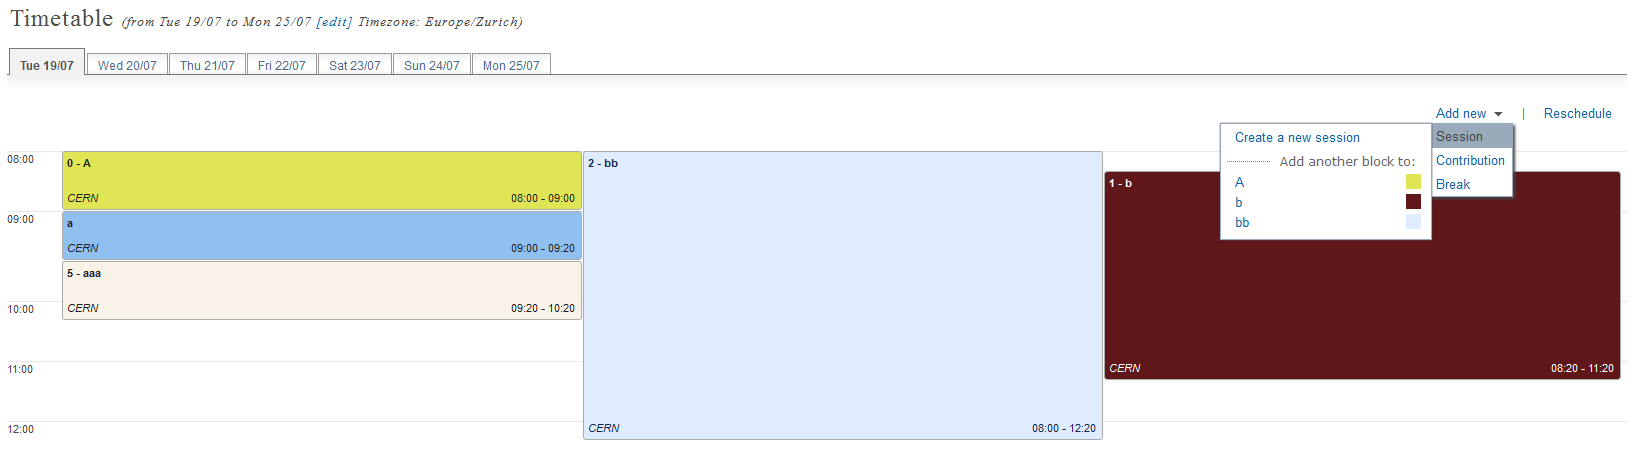
\includegraphics[scale=0.3]{indico_timetable.png}
			\end{center}
			\caption[Timetable in Indico (esempio)]{Un esempio di timetable di una conferenza in Indico (fonte \cite{indico:user_guide_1.9.6}).}
			\label{fig:indico_timetable}
		\end{figure}
		
		\paragraph{UI}Indico utilizza anche una potente e immediata interfaccia utente che si basa sul design \acr{WYSIWYG}. Grazie a questa \acr{UI} sarà facilissimo eseguire azioni altrimenti più complesse e tediose: la definizione di un form di registrazione per l'evento, la gestione delle timetable, che implementano un'intuitiva interfaccia drag-and-drop, oppure editor di testo che permettono l'utilizzo di rich text o formule matematiche.
		
		\paragraph{Struttura}Indico, ed il suo sistema di protezione, sono organizzati in una struttura ad albero per categorie. Indico è stato sviluppato principalmente per grandi aziende, per questo gli eventi, ed il materiale ad essi associato, sono organizzati secondo una struttura gerarchica di categorie. L'amministratore del sistema potrà decidere ed assegnare livelli di protezione alle varie categorie secondo diversi livelli di granularità.

		\begin{figure}[h!]
			\begin{center}
				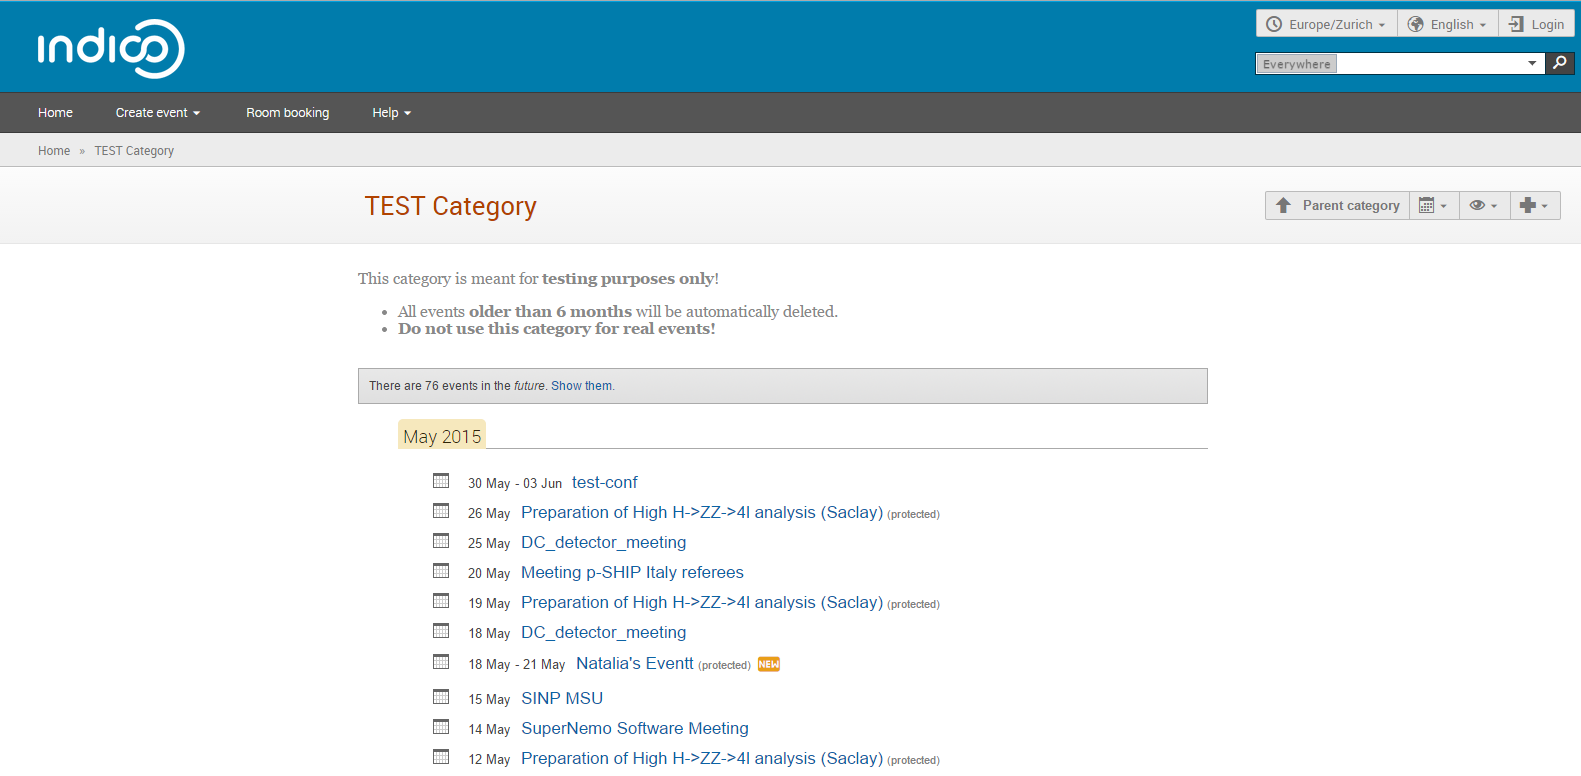
\includegraphics[scale=0.3]{indico_category.png}
			\end{center}
			\caption[Categoria in Indico (esempio)]{Un esempio di categoria con una serie di eventi al suo interno (fonte \cite{indico:user_guide_1.9.6}).}
			\label{fig:indico_category}
		\end{figure}
		
		\paragraph{Ricerca}In Indico è incluso anche un potente sistema di ricerca, che permette di ricercare gli eventi desiderati tramite poche parole chiave o osservare gli eventi previsti per un determinato periodo di tempo. Inoltre, tramite la dashboard, è possibile accedere velocemente a tutti gli eventi a cui l'utente è iscritto o che sta osservando.
		
		\paragraph{Room booking}Le compagnie e le organizzazioni, specialmente le più grandi, hanno spesso bisogno di gestire, limitare e tener traccia dell'utilizzo delle varie stanze e siti al loro interno. Per questo Indico include un potente ed intuitivo modulo per la prenotazione delle stanza (in inglese, \textit{Room Booking}) che permette all'utente di specificare le caratteristiche di una stanza, approvare o meno la prenotazione di certe stanze e gestire strumenti e materiale messi a disposizione da una certa stanza, come dispositivi audiovisivi per le video conferenze.
		
		Cliccando sulla voce ``Room Booking'' nel menu principale di Indico, si verrà portati alla schermata principale del modulo di Room Booking, come possiamo vedere in Figura \ref{fig:rb_booking_a_room}.
		
		\begin{figure}[h!]
			\begin{center}
				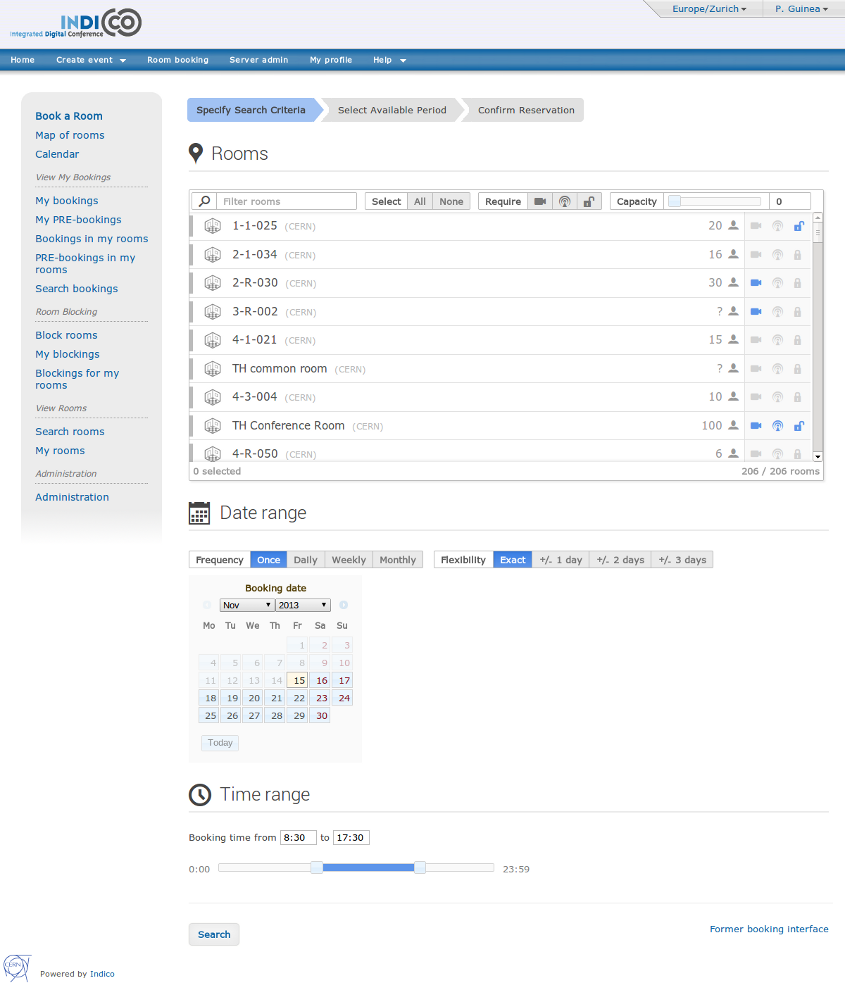
\includegraphics[scale=0.4]{rb_booking_a_room.png}
			\end{center}
			\caption[Room Booking in Indico]{Interfaccia del modulo di Room Booking di Indico (fonte \cite{indico:user_guide_1.9.6}).}
			\label{fig:rb_booking_a_room}
		\end{figure}
		
		L'esempio in Figura \ref{fig:rb_booking_a_room} mostra chiaramente quanto sia intuitiva l'interfaccia di Indico: in questo caso è possibile ricercare una o più stanze e selezionare varie date o intervalli di tempo in modo semplice grazie all'interfaccia molto moderna di questo modulo. Un altro esempio, in questo frangente, della potenza dell'interfaccia di Indico, è dato dalla Figura \ref{fig:rb_conflicts}.
		
		\begin{figure}[h!]
			\begin{center}
				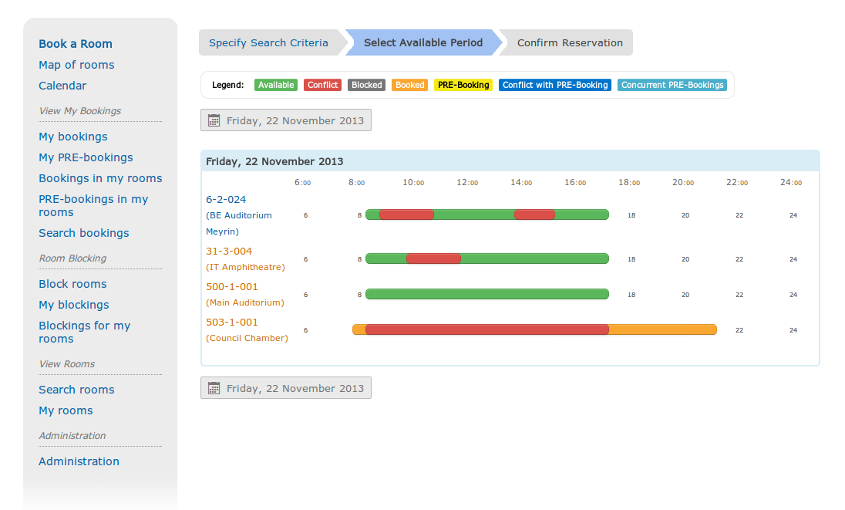
\includegraphics[scale=0.4]{rb_conflicts.png}
			\end{center}
			\caption[Conflitto di date con Room Booking]{Esempio di conflitto tra date nel modulo Room Booking (fonte \cite{indico:user_guide_1.9.6}).}
			\label{fig:rb_conflicts}
		\end{figure}
		
		La schermata in Figura \ref{fig:rb_conflicts} rappresenta lo step successivo all'esempio in Figura \ref{fig:rb_booking_a_room}, ovvero una volta selezionate stanze, date e orari, e mostra come vengono visualizzate le date e orari disponibili per le stanze scelte, evidenziando, eventualmente, i conflitti presenti con altre prenotazioni già effettuate.
		
		\paragraph{Chat \& Video}Per rendere la gestione online di riunioni e conferenze ancora più efficiente, Indico integra perfettamente Vidyo\footnote{\url{http://it.vidyo.com/}.}, uno strumento per le videoconferenze, e permette di associare delle chatrooms Jabber/XMPP agli eventi.

		\begin{figure}[h!]
			\begin{center}
				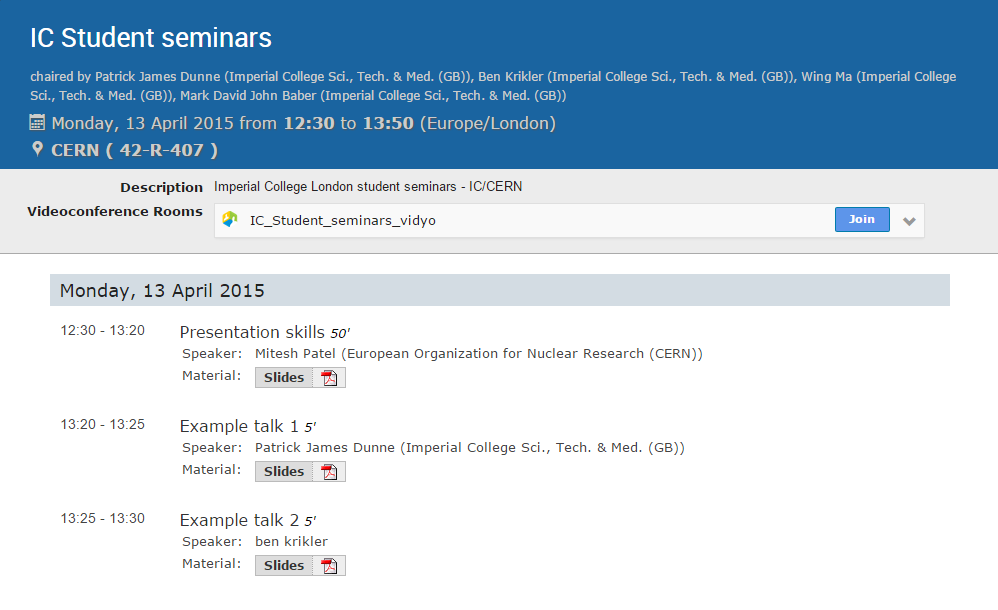
\includegraphics[scale=0.5]{indico_meeting.png}
			\end{center}
			\caption[Meeting in Indico (esempio)]{Un esempio di riunione in Indico con una videoconference room Vidyo associata (fonte \cite{indico:user_guide_1.9.6}).}
			\label{fig:indico_meeting}
		\end{figure}
		
		\paragraph{API}Dal momento che Indico è stato creato per agevolare la collaborazione e lo scambio di dati, tutte le informazioni contenute in Indico non sono esclusive di Indico stesso, ma possono essere recuperate (una volta accertato di avere l'accesso a quelle informazioni) tramite una semplice \acr{API}. Quest'\ac{API} è garantita essere RESTful  (dove \acs{REST} significa \aclu{REST}) ed è in costante aggiornamento.
		
	\section{Dettagli tecnici} \label{sec:i;dettagli_tecnici}
	
		Indico è un'applicazione web scritta principalmente in Python e Javascript (si veda la Figura \ref{fig:indico_languages}).
		
		\begin{figure}[h!]
			\begin{center}
				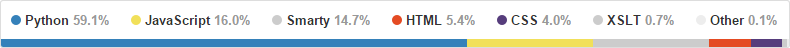
\includegraphics[scale=0.6]{indico_languages.png}
			\end{center}
			\caption[Linguaggi di Indico]{Una statistica dei linguaggi utilizzati nel codice di Indico (fonte GitHub).}
			\label{fig:indico_languages}
		\end{figure}
		
		Essendo un'applicazione web, Indico implementa un web server ed un \ac{DB} per gestire le richieste dell'utente e recuperare i dati richiesti.
		
		\paragraph{WSGI}Indico utilizza \acr{WSGI} per gestire il web server. \ac{WSGI} è un'interfaccia standard tra web server e applicazioni Python, ovvero un'astrazione per rendere la comunicazione tra le due parti più semplice e modulare. In questo modo il server e  l'applicazione sono completamente separati e seguono lo standard. Ad esempio per Indico@CERN si utilizza Apache come web server, ma un amministratore di un'altra istanza può scegliere un altro server se lo desidera, in quanto \ac{WSGI} si configura senza problemi con quasi tutti i web server in circolazione. \cite{indico:wsgi}
		
		\paragraph{DB}Prima dell'inizio del periodo di Techical Student, Indico utilizzava \acr{ZODB} come database. \ac{ZODB} è un database object-oriented che immagazzina oggetti Python. Dai primi del 2014 è invece stata iniziata una fase di migrazione, in  quanto \ac{ZODB} presentava alcuni svantaggi, come la difficoltà di eseguire query, la non indicizzazione dei record e il fatto di poter essere utilizzabile soltanto con Python. Dopo alcuni mesi di ricerca su quale potesse essere il miglior candidato per sostituire \ac{ZODB}, si è scelto PostgreSQL (spesso detto Postgres) come vincitore. Postgres è un \acr{ORDBMS}, ovvero un database relazionale a oggetti, che garantirà prestazioni più elevate durante l'utilizzo di Indico. Ovviamente passare da un database ad un altro non è una cosa semplice, in quanto tutto il codice dove si comunica con il \ac{DB} dev'essere adeguato al nuovo database. Migrare l'intero \ac{DB} di Indico@CERN in un sol colpo era quindi un'impresa del tutto non fattibile. Si è optato quindi per una migrazione modulare: il processo di migrazione durerà circa un anno, durante il quale Indico utilizzerà un sistema di gestione del \ac{DB} ibrido \ac{ZODB}+Postgres, migrando modulo per modulo. \cite{indico:zodb}\cite{pedro:chep}
		
		\paragraph{Flask}Flask è un micro framework per applicazioni web, scritto in Python e basato su Werkzeug e Jinja2. Uno dei principali vantaggi offerti da Flask è l'\acr{URL} routing, ovvero la  possibilità di gestire gli \ac{URL} in modo dinamico. Si possono associare diversi template per ogni tipo di richiesta ricevuta dal server, in modo da generare una pagina dinamica a seconda degli argomenti passati da Flask al template engine. \cite{indico:flask}
		
		\paragraph{Template engine(s)}Un template engine è uno strumento che permette di creare documenti personalizzati e dinamici a partire da un template (ovvero un modello) di base e dei parametri di input. In questo caso, quando si parla di template engines, ci si riferisce a strumenti che generano pagine web secondo un certo modello inserendovi dei dati dinamici. Indico ha utilizzato per molti anni Mako come template engine ma in questi ultimi anni sta lentamente passando a Jinja2. \cite{indico:template_engines}
		
		\paragraph{Altre}A parte queste tecnologie citate, Indico ha iniziato a impiegare, nel corso degli ultimi anni, altri strumenti degni di nota, come  ad esempio WTForms, per la gestione dei campi dei form (ad esempio form di registrazione), SQLAchemy, ovvero un toolkit open source SQL, ed Alembic, uno strumento per la migrazione di database da utilizzare con SQLAlchemy.
		
	\section{La community} \label{sec:i;community}
	
		Come già accennato,  Indico è un software open source. Il suo codice sorgente più aggiornato è infatti disponibile su GitHub, all'indirizzo \url{https://github.com/indico/indico}. Il fatto di essere open source ha portato centinaia di organizzazioni e istituzioni, soprattutto nel campo della fisica delle particelle come ad esempio \acr{INFN} e \acr{IHEP}, ad utilizzare Indico per la gestione dei propri eventi. Negli anni questo ha portato alla formazione di una vera e propria community di utilizzatori (user e admin) di Indico.
		
		Questa community non soltanto utilizza Indico per i propri eventi, ma contribuisce anche allo sviluppo stesso del software,  inviando segnalazioni agli sviluppatori del team Indico  al \ac{CERN} sotto forma di ticket. Un ticket indica un problema da risolvere, o qualcosa da migliorare; risolvere il problema in questione o apportare la miglioria richiesta viene indicato con il termine di ``chiusura del ticket''.
		
		Altre volte invece, se chi si imbatte in un errore è uno sviluppatore a sua volta, può capitare che provi a risolvere il problema da solo, lavorando sul codice di Indico. Una volta  risolto, chi ha risolto il problema può inviare una cosiddetta \textit{pull request} tramite GitHub (il repository ufficiale che ospita il codice di Indico) agli sviluppatori di Indico al \ac{CERN}, in modo da indicare che  quel  problema è già stato risolto e possono includere (operazione di \textit{merge}) le modifiche apportate al codice principale di Indico.
	